% -*- compile-command: "cd ../ && make" -*-
\eocesolch{Distributions of random variables}

\begin{multicols}{2}

% 1

\eocesol{(a)~8.85\%.
(b)~6.94\%.
(c)~58.86\%.
(d)~4.56\%. \\
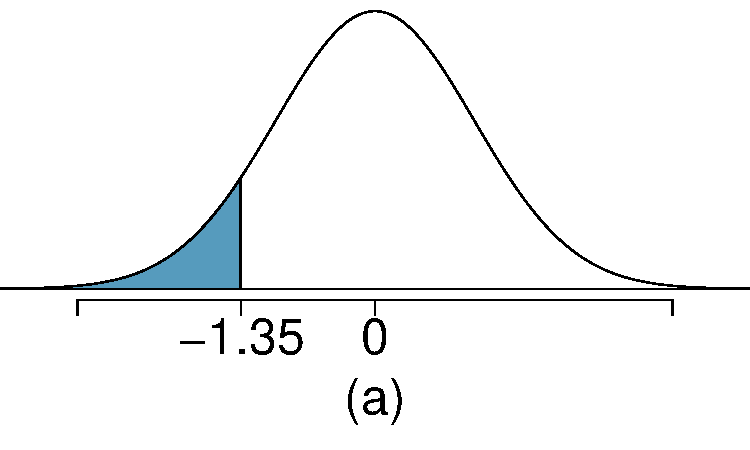
\includegraphics[width=0.23\textwidth]{ch_distributions/figures/eoce/area_under_curve_1/zltNeg}
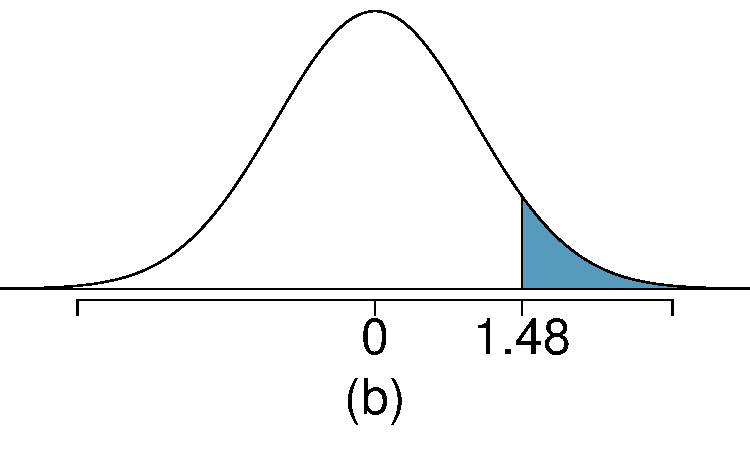
\includegraphics[width=0.23\textwidth]{ch_distributions/figures/eoce/area_under_curve_1/zgtPos}
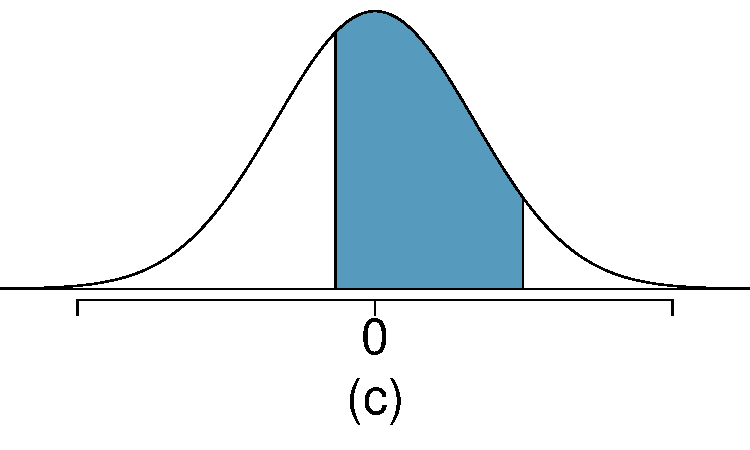
\includegraphics[width=0.23\textwidth]{ch_distributions/figures/eoce/area_under_curve_1/zBet}
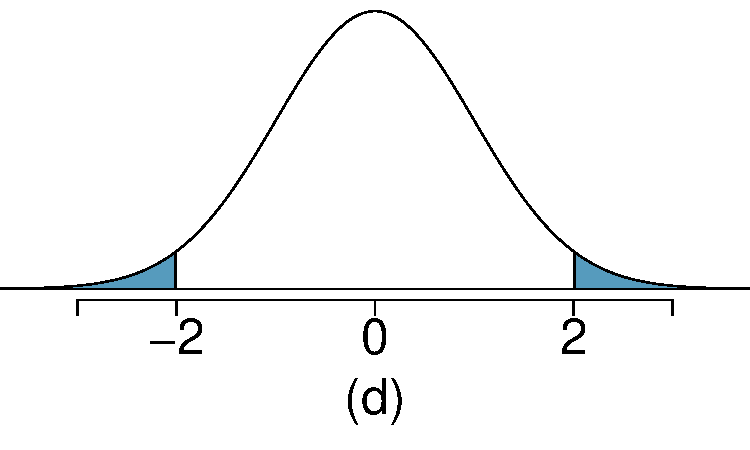
\includegraphics[width=0.23\textwidth]{ch_distributions/figures/eoce/area_under_curve_1/zgtAbs}}

% 3

\eocesol{(a)~Verbal: $N(\mu = 151, \sigma = 7)$, Quant: $N(\mu = 153, \sigma = 7.67)$.
(b)~$Z_{VR} = 1.29$, $Z_{QR} = 0.52$. \\
\includegraphics[width=0.3\textwidth]{ch_distributions/figures/eoce/GRE_intro/GRE_intro.pdf} \\
(c)~She scored 1.29 standard deviations above the mean on the Verbal
Reasoning section and 0.52 standard deviations above the mean on the
Quantitative Reasoning section.
(d)~She did better on the Verbal Reasoning section since her Z-score on that
section was higher.
(e)~$Perc_{VR} = 0.9007 \approx 90\%$, $Perc_{QR} = 0.6990 \approx 70\%$.
(f)~$100\% - 90\% = 10\%$ did better than her on VR, and $100\% - 70\% = 30\%$
 did better than her on QR.
(g)~We cannot compare the raw scores since they are on different scales.
Comparing her percentile scores is more appropriate when comparing her
performance to others.
(h)~Answer to part (b) would not change as Z-scores can be calculated for
distributions that are not normal. However, we could not answer parts~(d)-(f)
since we cannot use the normal probability table to calculate probabilities
and percentiles without a normal model.}

% 5

\eocesol{(a)~$Z = 0.84$, which corresponds to approximately 160 on QR.
(b)~$Z = -0.52$, which corresponds to approximately 147 on VR.}

% 7

\eocesol{(a)~$Z=1.2 \to 0.1151$. \\
(b)~$Z= -1.28 \to 70.6\degree$F or colder.}



\textC{
\end{multicols}
\newpage
\begin{multicols}{2}
}



% 9

\eocesol{(a)~$N(25, 2.78)$.
(b)~$Z = 1.08 \to 0.1401$.
(c)~The answers are very close because only the units were changed. (The only
reason why they differ at all is because 28\degree C is
82.4\degree F, not precisely 83\degree F.)
(d)~Since $IQR = Q3 - Q1$, we first need to find $Q3$ and $Q1$ and take the
difference between the two. Remember that $Q3$ is the $75^{th}$ and $Q1$ is
the $25^{th}$ percentile of a distribution. Q1 = 23.13, Q3 = 26.86, IQR = 26.
86 - 23.13 = 3.73.}

% 11

\eocesol{(a)~$Z=0.67$.
(b)~$\mu=\$1650$, $x=\$1800$.
(c)~$0.67 = \frac{1800-1650}{\sigma} \to \sigma=\$223.88$.}

% 13

\eocesol{$Z = 1.56 \to 0.0594$, i.e. 6\%.}

% 15

\eocesol{(a)~$Z=0.73 \to 0.2327$.
(b)~If you are bidding on only one auction and set a low maximum bid price,
someone will probably outbid you. If you set a high maximum bid price, you
may win the auction but pay more than is necessary. If bidding on more than
one auction, and you set your maximum bid price very low, you probably won't
win any of the auctions. However, if the maximum bid price is even modestly
high, you are likely to win multiple auctions.
(c)~An answer roughly equal to the 10th percentile would be reasonable.
Regrettably, no percentile cutoff point guarantees beyond any possible event
that you win at least one auction. However, you may pick a higher percentile
if you want to be more sure of winning an auction.
(d)~Answers will vary a little but should correspond to the answer in
part~(c). We use the 10$^{th}$ percentile: $Z = -1.28 \to \$69.80$.}

% 17

\eocesol{(a)~70\% of the data are within 1 standard deviation of the mean, 95\% are
within 2 and 100\% are within 3 standard deviations of the mean. Therefore,
we can say that the data approximately follow the 68-95-99.7\% Rule.
(b)~The distribution is unimodal and symmetric. The superimposed normal
curve seems to approximate the distribution pretty well. The points on the
normal probability plot also seem to follow a straight line. There is one
possible outlier on the lower end that is apparent in both graphs, but it is
not too extreme. We can say that the distribution is nearly normal.}

% 19

\eocesol{(a)~No. The cards are not independent. For example, if the first card is an
ace of clubs, that implies the second card cannot be an ace of clubs.
Additionally, there are many possible categories, which would need to be
simplified.
(b)~No. There are six events under consideration. The Bernoulli distribution
allows for only two events or categories. Note that rolling a die could be a
Bernoulli trial if we simply to two events, e.g. rolling a 6 and not rolling
a 6, though specifying such details would be necessary.}

% 21

\eocesol{(a)~$(1-0.471)^2\times0.471 = 0.1318$.
(b)~$0.471^3 = 0.1045$.
(c)~$\mu = 1/0.471 = 2.12$, $\sigma=\sqrt{2.38} = 1.54$.
(d)~$\mu = 1/0.30 = 3.33$, $\sigma=2.79$.
(e)~When $p$ is smaller, the event is rarer, meaning the expected number of
trials before a success and the standard deviation of the waiting time are
higher.}

% 23

\eocesol{(a)~$0.875^2\times 0.125 = 0.096$. \\
(b)~$\mu=8$, $\sigma=7.48$.}

% 25

\eocesol{(a)~Binomial conditions are met:
(1)~Independent trials: In a random sample, whether or not one 18-20 year
old has consumed alcohol does not depend on whether or not another one has.
(2)~Fixed number of trials: $n = 10$.
(3)~Only two outcomes at each trial: Consumed or did not consume alcohol.
(4)~Probability of a success is the same for each trial: $p = 0.697$.
(b)~0.203.
(c)~0.203.
(d)~0.167.
(e)~0.997.}

% 27

\eocesol{(a)~$\mu = 34.85$, $\sigma = 3.25$
(b)~$Z = \frac{45 - 34.85}{3.25} = 3.12$. 45 is more than 3 standard
deviations away from the mean, we can assume that it is an unusual
observation. Therefore yes, we would be surprised.
(c)~Using the normal approximation, 0.0009. With 0.5 correction, 0.0015.}

% 29

\eocesol{Want to find the probability that there will be 1,786 or more enrollees.
Using the normal approximation: 0.0582. With a 0.5 correction: 0.0559.}

% 31

\eocesol{(a)~$1-0.75^3 = 0.5781$.
(b)~0.1406.
(c)~0.4219.
(d)~$1-0.25^3=0.9844$.}

% 33

\eocesol{(a)~Geometric distribution: 0.109.
(b)~Binomial: 0.219.
(c)~Binomial: 0.137.
(d)~$1-0.875^6=0.551$.
(e)~Geometric: 0.084.
(f)~Using a binomial distribution with $n = 6$ and $p=0.75$, we see that $\mu=4.5$, $\sigma=1.06$, and $Z = 2.36$. Since this is not within 2 SD, it may be considered unusual.}

% 35

\eocesol{0 wins (-\$3): 0.1458. 1 win (-\$1): 0.3936. 2 wins (+\$1): 0.3543.
3 wins (+\$3): 0.1063.}


\textC{
\end{multicols}
\newpage
\begin{multicols}{2}
}


% 37

\eocesol{(a)~$\stackrel{Anna}{1/5}\times\stackrel{Ben}{1/4}\times\stackrel{Carl}{1/3}\times\stackrel{Damian}{1/2}\times\stackrel{Eddy}{1/1} = 1/5!=1/120$.
(b)~Since the probabilities must add to 1, there must be $5!=120$ possible orderings.
(c)~$8!=\text{40,320}$.}

% 39

\eocesol{(a)~0.0804.
(b)~0.0322.
(c)~0.0193.}

% 41

\eocesol{(a)~Negative binomial with $n=4$ and $p=0.55$, where a success is defined here as a female student. The negative binomial setting is appropriate since the last trial is fixed but the order of the first 3 trials is unknown.
(b)~0.1838.
(c)~${3 \choose 1} = 3$.
(d)~In the binomial model there are no restrictions on the outcome of the last trial. In the negative binomial model the last trial is fixed. Therefore we are interested in the number of ways of orderings of the other $k - 1$ successes in the first $n - 1$ trials.}

% 43

\eocesol{(a)~Poisson with $\lambda=75$.
(b)~$\mu=\lambda=75$, $\sigma=\sqrt{\lambda} = 8.66$.
(c)~$Z=-1.73$. Since 60 is within 2 standard deviations of the mean, it would not generally be considered unusual. Note that we often use this rule of thumb even when the normal model does not apply.
(d)~Using Poisson with $\lambda = 75$: 0.0402.}



%_______________
\end{multicols}
